\section{Catalisi delle reazioni}
\diapo{Due possibili meccanismi di reazione}
\begin{figure}{\centering{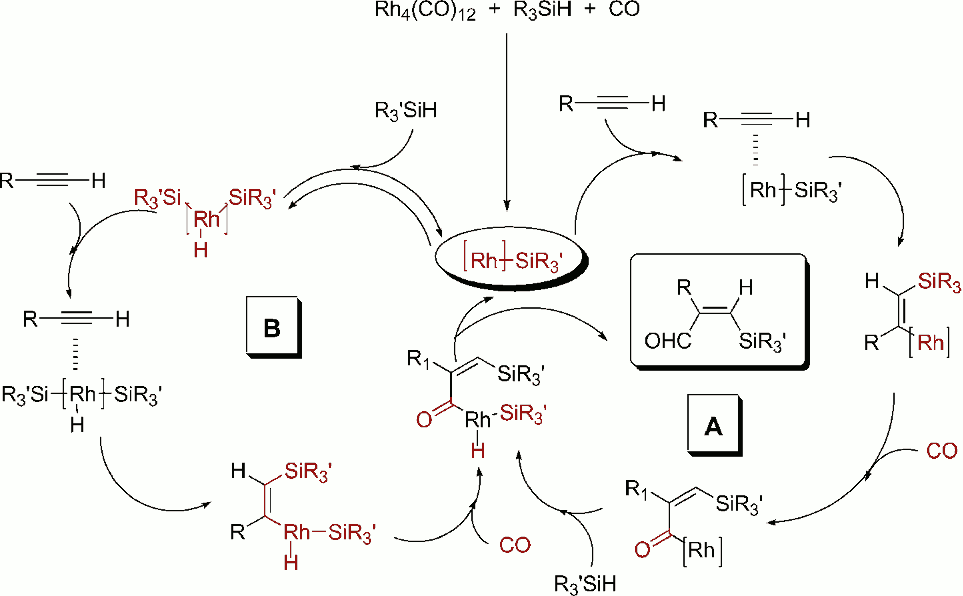
\includegraphics[width=0.9\textwidth]{img/catalisi/cicli.png}}}\end{figure}

\end{frame}
\subsubsection{Quantità di catalizzatore}\begin{frame}\frametitle{Due possibili meccanismi di reazione}\framesubtitle{Quantità di catalizzatore}
\begin{columns}
\column{0.45\linewidth}
Una {\bf eccessiva quantità di catalizzatore favorisce la idrosililazione}. 

Sembra che la grande quantità di catalizzatore renda più efficiente l'eliminazione riduttiva rispetto all'inserimento di \ce{CO}. 
\column{0.5\linewidth}\begin{figure}{\centering{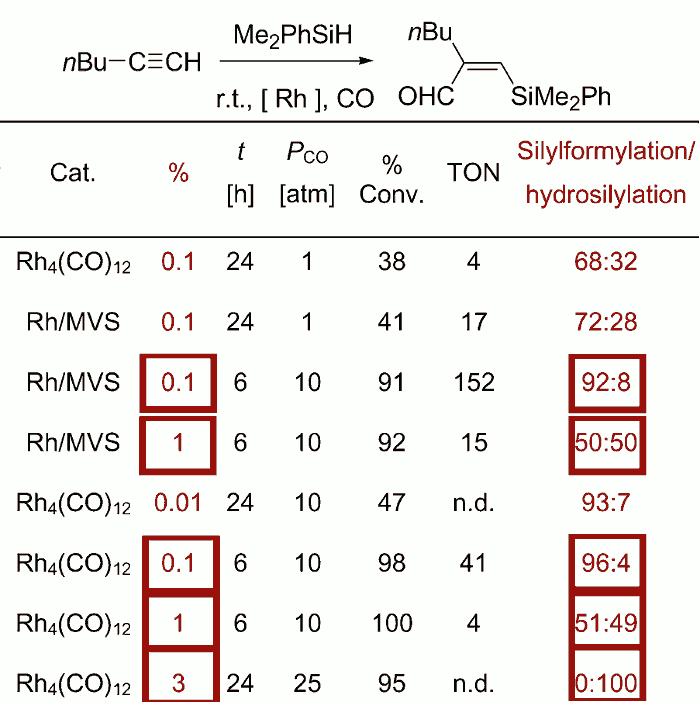
\includegraphics[width=0.9\textwidth]{img/catalisi/quantcat.png}}}\end{figure}
\end{columns}


\end{frame}
\logo{}
\diapo{Catalizzatori ``tradizionali''}
Sono stati {\bf testati numerosi catalizzatori} per la reazione di {\bf sililformilazione}:
\begin{figure}{\centering{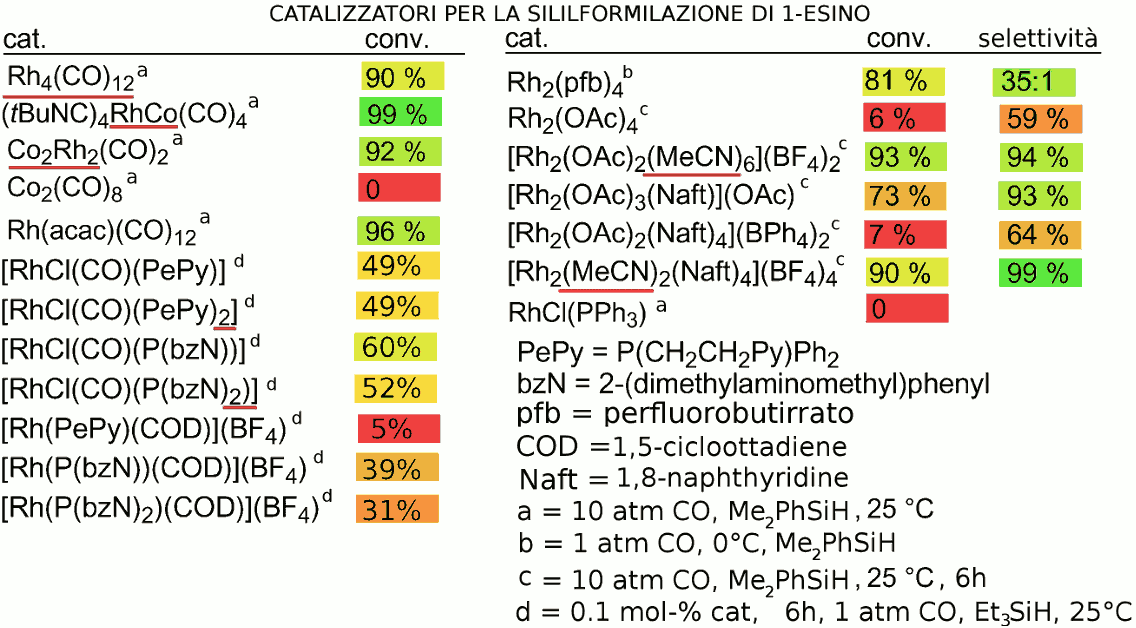
\includegraphics[width=1\textwidth]{img/catalisi/catalizzatori.png}}}\end{figure}

\end{frame}
\logo{
\includegraphics[width=0.07\paperwidth]{img/snslogo.png}}

%%%%%%%%%%%%%%%%%%%%%%%%%%%%%%%%%%%%%%%%%%%%%%%%%%%%%%%%%%%%%%%%%%%%

\diapo{Catalizzatori realizzati con MVS}
Tramite tecnica {\bf Metal Vapour Synthesis} sono stati preparati catalizzatori {\bf supportati} o nanocluster di rodio (stabili in mesitilene solo a -40\textdegree C).
\begin{figure}{\centering{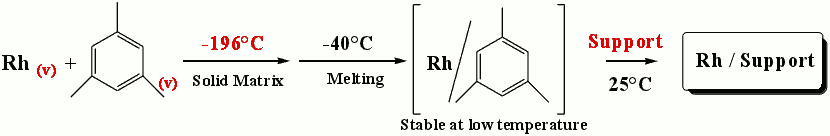
\includegraphics[width=1\textwidth]{img/catalisi/mvs.png}}}\end{figure}
Il supporto è stato utilizzato sia per avere una stabilità maggiore sia per ottenere una catalisi eterogenea. 
\pause

Purtroppo s'è riscontrato che {\bf la catalisi avviene omogenea} da parte di rodio liberatosi dal supporto.
\end{frame}
\definecolor{orange}{RGB}{255,160,0}

\subsubsection{Risultati}\begin{frame}\frametitle{Catalizzatori realizzati con MVS}\framesubtitle{Risultati}
I {\bf catalizzatori MVS danno attività specifiche maggiori} rispetto al riferimento \ce{Rh4(CO)12}.


 \pause {\bf Supporti molto polari liberano meno particelle} ed hanno efficacie minori. 
{\bf Catalizzatori supportati commerciali} hanno efficacia quasi {\bf nulla} a causa della {\bf dimensione delle nanoparticelle molto maggiore}. 
{\footnotesize\begin{center}
   \begin{tabular}{c c c}
\multicolumn{3}{c}{Sililformilazione di 1-esino} \\
\multicolumn{3}{c}{{\tiny(t=6h, 2mmol \ce{Me2OhSiH}, 2mmol 1-esino, 2$\mu$mol Rh, 2mL toluene, 25\textdegree C, 10atm CO)}} \\
 Catalizzatore & Conversione (\%) & Selettività (\%) \\
\midrule
\ce{Rh4(CO)12} & \color{green}98 & \color{green}96 \\
\ce{Rh$/$Mesitilene} & \color{yellow} 91 & \color{yellow}92 \\
\ce{Rh$/$C (MVS)} & \color{orange}81 & \color{yellow}94 \\
\ce{Rh$/$Fe2O3 (MVS)} & \color{red}43 & \color{green}97 \\
\ce{Rh$/$C (commerciale)} & \color{red}12 & \color{green}97
   \end{tabular}
  \end{center}}
\end{frame}
%%%%%%%%%%%%%%%%%%%%%%%%%%%%%%%%%%%%%%%%%%%%%%%%%%%%%%%%%%%%%%%%%%%%
\AtBeginSection[]{\frame{\tableofcontents[current,hideothersubsections,subsubsectionstyle=hide]}}
